\section{Evaluation and Discussion}
\label{sec:discussion}

One of the design goals of Vivian is to let IoT devices be able to use client software for naming operations and file storage.
For naming operations, client software needs to handle transactions on Tangle and communicate with nodes in peer network layer.
We evaluate the compatibility of the naming operations on IoT devices by testing the performance of sending and reading IOTA transactions on devices with limited hardware resources.
The devices used for performance evaluations are:

\begin{enumerate}
    \item Raspberry Pi Zero W: 
        \begin{itemize}
            \item Hardware: 802.11 b/g/n wireless LAN, 1GHz single-core CPU (ARMv6 architecture), 512MB RAM, with 16GB SD card.
            \item Software: Raspberry Pi OS Lite.
        \end{itemize}
    \item Raspberry Pi 4 B: 
    \begin{itemize}
        \item Hardware: 2.4 GHz and 5.0 GHz IEEE 802.11ac wireless,  1.5GHz quad core Cortex-A72 (ARM v8) 64-bit CPU, 4GB RAM, with 16GB SD card.
        \item Software: Ubuntu Server 20.04.2 LTS.
    \end{itemize}
\end{enumerate}

We prepared two sets of program for the test: sending transactions and reading transactions. They are all written in Golang (v 1.16) based on \texttt{iota.go}, the official Golang library for IOTA.
Sending transaction program will generate a new seed and continuously send zero-value transaction for 100 times, there is 10 seconds' delay between each sending operation.
There are three steps for each sending operation: getting new address, preparing transfer for creating a bundle in trytes, and sending trytes which handles tip selection, remote proof of work, and sending the bundle to the node.
Please note that proof-of-work procedure here is different from PoW consensus mechanism in Bitcoin, it is a method for preventing spam in the network, and the workload is much less than PoW in Bitcoin.
Reading transaction program will continuously read transactions according to different tail transaction hash for 100  times, there is 10 seconds' delay between each reading operation.
There are two steps for each reading operation: getting the bundle to get all transactions in the tail transaction's bundle, and extracting JSON to decode the JSON messages in the signatureMessageFragment fields of the transactions.
The programs measure the cost of each procedure by recording the execution time.

\begin{figure}[h]
    \centering
    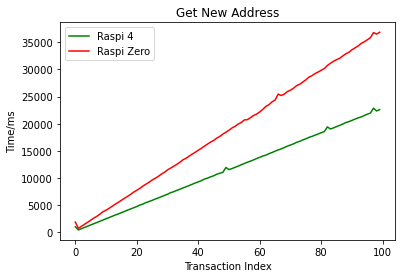
\includegraphics[width=0.4\textwidth,trim={0 0 0 0},clip]{figs/get_new_address.png}
    \caption{Cost of getting new address procedure}
    \label{fig:cost_getting_new_address}
\end{figure}

The first step of sending a transaction is getting a new unspent address generated by user's private seed.
From the result of cost of getting new address, we noticed that the time taken for getting a new unspent address is increasing significantly. 
We analyzed the possible reason for this result. The test program uses API \texttt{getNewAddress()} to generate new addresses, it will first generate new addresses with private seed locally and request IOTA nodes for checking if the address is a spent from a given index.
If the address with given index if spent, the index in incremented until the nodes find an unspent address. As number of unspent addresses is increasing, time taken for finding an unspent one becomes longer. 
We will consider keeping track of spent addresses on local database for better management to reduce new address generation time in real implementation.

% \begin{figure}[h]
%     \centering
%     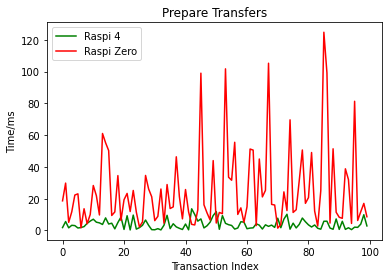
\includegraphics[width=0.3\textwidth,trim={0 0 0 0},clip]{figs/prepare_transfers_0.png}
%     \caption{Cost of preparing transfers}
%     \label{fig:cost_preparing_transfers}
% \end{figure}

% \begin{figure}[h]
%     \centering
%     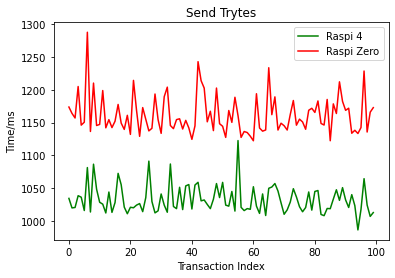
\includegraphics[width=0.3\textwidth,trim={0 0 0 0},clip]{figs/send_trytes_0.png}
%     \caption{Cost of sending trytes}
%     \label{fig:cost_sending_trytes}
% \end{figure}

% \begin{figure}[h]
%     \centering
%     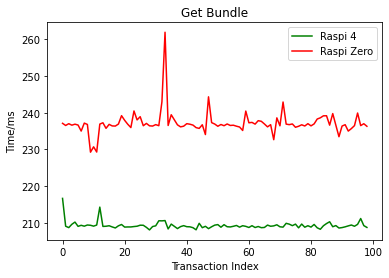
\includegraphics[width=0.3\textwidth,trim={0 0 0 0},clip]{figs/get_bundle_0.png}
%     \caption{Cost of getting bundle}
%     \label{fig:cost_getting_bundle}
% \end{figure}

From the result of getting the bundle of transactions, we found that the time taken for the first request is much longer than the others. We think it is possibly due to IOTA node's orientation process from a new device.
Fig~\ref{fig:cost_getting_bundle} shows the time cost of the remaining 99 requests.

% \begin{figure}[h]
%     \centering
%     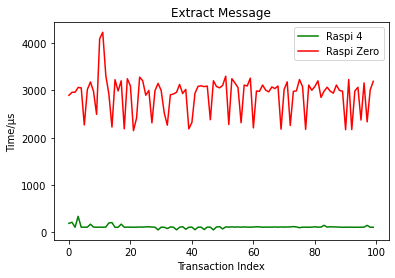
\includegraphics[width=0.3\textwidth,trim={0 0 0 0},clip]{figs/extract_message_0.png}
%     \caption{Cost of extracting JSON}
%     \label{fig:cost_extracting_json}
% \end{figure}


\begin{figure*}[t]
    \centering

\begin{minipage}[t]{0.45\linewidth}
    \centering
    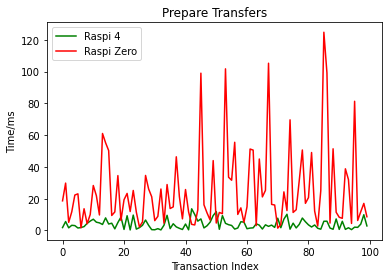
\includegraphics[width=0.8\textwidth]{figs/prepare_transfers_0.png}
    \caption{Cost of preparing transfers}
    \label{fig:cost_preparing_transfers}
\end{minipage}
		\hfill
\begin{minipage}[t]{0.45\linewidth}
    \centering
    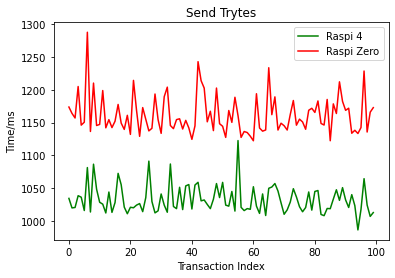
\includegraphics[width=0.8\textwidth]{figs/send_trytes_0.png}
    \caption{Cost of sending trytes}
    \label{fig:cost_sending_trytes}
\end{minipage}		
\\ [1ex]
\begin{minipage}[t]{0.45\linewidth}
    \centering
    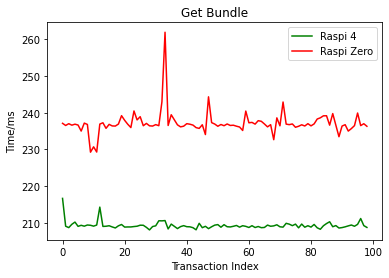
\includegraphics[width=0.8\textwidth]{figs/get_bundle_0.png}
    \caption{Cost of getting bundle}
    \label{fig:cost_getting_bundle}
    \end{minipage}
    \hfill
\begin{minipage}[t]{0.45\linewidth}
    \centering
    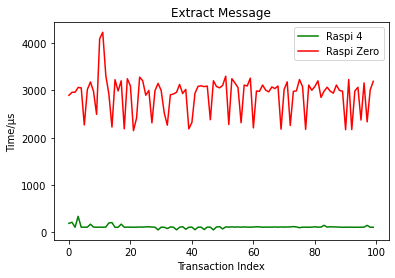
\includegraphics[width=0.8\textwidth]{figs/extract_message_0.png}
    \caption{Cost of extracting JSON}
    \label{fig:cost_extracting_json}
\end{minipage}
\end{figure*}

In summary, with Raspberry Pi 4, the mean time of sending a transaction (excluding getting new addresses) is 1037ms, and mean time for reading a transaction is 217ms. 
With Raspberry Pi Zero, the mean time of sending a transaction (excluding getting new addresses) is 1187ms, and mean time for reading a transaction is 255ms. 
We think this performance is good enough for real use cases in IoT services.

Due to the complexity of peer network communication and file storage, detailed evaluations are left for future work.

In this work, we proposed a decentralized approach for the current Internet services and Domain Name System to enhance better security and user data security.
By removing central trust parties, the system has no single-point failure and users can register human-meaningful names without relying on the trust of third parties.
The system also provides an alternative storage layer for a decentralized and secure storage of user data.
Decentralized naming system has been proposed for a long time and there are already existing implementations like Namecoin \cite{kalodner2015empirical}, Blockstack BNS \cite{ali2017blockstack} and Ethereum ENS\footnote{ENS: Ethereum Naming System. Documents: \url{https://docs.ens.domains/}}. However, these systems rely on PoW blockchains that require miners and huge energy consumption for Proof-of-Work consensus.
Transaction fees need to be paid for miners' work.
Also, the blockchains they are relying on are also facing scalability, low TPS and long transaction validation time issues.
Instead, in our system, we decide to adopt another type of distributed ledger, DAG, for solving these issues. In addition, there is no miners in the network and confirming a transaction does not require much computational work. This makes the system more economical and environmentally friendly. Its high scalability, feeless, and lightweight characteristics also enables the ability of extending the system features on IoT devices.

Besides the design and implementation of the system included in this paper, there are more topics to be cover in the future: incentive to run a node in the peer network layer, pricing function for a name, how to ease node eclipse attack \cite{singh2006eclipse}, etc.
